\documentclass{article}

% if you need to pass options to natbib, use, e.g.:
% \PassOptionsToPackage{numbers, compress}{natbib}
% before loading nips_2016
%
% to avoid loading the natbib package, add option nonatbib:
% \usepackage[nonatbib]{nips_2016}

\usepackage{nips_2016}

% to compile a camera-ready version, add the [final] option, e.g.:
% \usepackage[final]{nips_2016}

\usepackage[utf8]{inputenc} % allow utf-8 input
\usepackage[T1]{fontenc}    % use 8-bit T1 fonts
\usepackage{hyperref}       % hyperlinks
\usepackage{url}            % simple URL typesetting
\usepackage{booktabs}       % professional-quality tables
\usepackage{amsfonts}       % blackboard math symbols
\usepackage{nicefrac}       % compact symbols for 1/2, etc.
\usepackage{microtype}      % microtypography
\usepackage{subfig}
\usepackage{amsmath}
\usepackage[pdftex]{graphicx}
% declare the path(s) where your graphic files are
\graphicspath{{pic/}}
% and their extensions so you won't have to specify these with
% every instance of \includegraphics
\DeclareGraphicsExtensions{.pdf}
\title{STDP Training on Spiking Autoencoders}

% The \author macro works with any number of authors. There are two
% commands used to separate the names and addresses of multiple
% authors: \And and \AND.
%
% Using \And between authors leaves it to LaTeX to determine where to
% break the lines. Using \AND forces a line break at that point. So,
% if LaTeX puts 3 of 4 authors names on the first line, and the last
% on the second line, try using \AND instead of \And before the third
% author name.

\author{
  Qian Liu and Steve Furber\thanks{} \\
  Advanced Processor Technologies group, School of Computer Science,\\
  University of Manchester, M13 9PL, Manchester, United Kingdom\\
  \texttt{qian.liu-3@manchester.ac.uk and steve.furber@manchester.ac.uk} \\
  %% examples of more authors
  %% \And
  %% Coauthor \\
  %% Affiliation \\
  %% Address \\
  %% \texttt{email} \\
  %% \AND
  %% Coauthor \\
  %% Affiliation \\
  %% Address \\
  %% \texttt{email} \\
  %% \And
  %% Coauthor \\
  %% Affiliation \\
  %% Address \\
  %% \texttt{email} \\
  %% \And
  %% Coauthor \\
  %% Affiliation \\
  %% Address \\
  %% \texttt{email} \\
}

\begin{document}
% \nipsfinalcopy is no longer used

\maketitle

\begin{abstract}
	How the brain works still remains a mystery and attracts researchers from various areas attempting to understand it.
	Nowadays, the exciting reports of the beating-human visual recognition and decision making have brought deep learning into the spotlight.
	It provides a clue which may unveil the mechanism of neural processing in the brain.
	Therefore, it becomes a hot topic to train and operate deep learning on spiking neural networks(SNN) underline the more biologically realistic way.
	This paper proposed a supervised learning rule to train the Autoencoders of spiking neurons using Spike-Timing-Dependent Plasticity (STDP).
	A network of two-layer Autoencoders was trained on the MNIST database with Integrate-and-Fire (IF) neurons.
	This results demonstrate the equivalent recognition capability comparing to the non-spiking implementations and validate the training ability of the learning rule .
	
\end{abstract}

\section{Introduction}
% no \IEEEPARstart
%\hfill mds
% 
%\hfill August 26, 2015
Deep Neural Networks (DNNs) are the most promising research field in computer vision, even exceeding human-level performance on image classification tasks~\cite{he2015delving}.
To investigate whether brains might work similarly on vision tasks, these powerful DNN models have been converted to spiking neural networks (SNNs).
In addition, the spiking DNN offers the prospect of neuromorphic systems that combine remarkable performance with energy-efficient training and operation.

Theoretical studies have shown that biologically-plausible learning, e.g. Spike-Timing-Dependent Plasticity (STDP), could approximate a stochastic version of powerful machine learning algorithms	~\cite{nessler2013bayesian,neftci2013event,neftci2013event,o2016deep}.
such as Expectation Maximization~\cite{nessler2013bayesian}, 
Contrastive Divergence~\cite{neftci2013event}, Markov Chain Monte Carlo~\cite{buesing2011neural} and Gradient Descent~\cite{o2016deep}.
Stochasticity, in contrast with the continuously differentiable functions used by ANNs, is intrinsic to the event-based spiking process, making network training difficult.

state-of-the-art of learning on SNN\cite{ponulak2010supervised,neftci2013event,burbank2015mirrored}

what's unique for the proposed method.

\section{Background Knowledge}
\subsection{Unsupervised Learning}
\subsubsection{Deep Learning}
\subsubsection{Autoencoders}
\subsubsection{Deep Belief Network}
Pre-trained with RBM.
\subsection{Spiking Neural Networks}
\subsubsection{Spiking Neurons}
\subsubsection{Coding Mechanism}
\subsubsection{Network of Spiking Neurons}
\subsection{STDP Learning}

\section{Methods}
%\subsection{Training Spiking Autoencoders}
%
%\subsection{Convergence Evaluation}
\subsection{Training Autoencoders}
%TODO rewording
Figure~\ref{fig:AE} shows a simplest architecture of an autoencoder, which is the same as a multilayer perceptron (MLP).
The only difference lies to the number of the output units, where an autoencoder has as many output neurons as the input.
In this example, the input layer feeds forward the data vector $\mathbf{v}$ to the hidden layer as weighted sum of the data, $\mathbf{net\_h}$.
Then the hidden units are activated by the input $\mathbf{net\_h}$ according to the activation function: $\mathbf{h}=\sigma(\mathbf{net\_h})$.
Finally, using the same approach the output of the network is generated, $\mathbf{v'}=\sigma(\mathbf{net\_v'})$, as the reconstruction of the input data.
Thus, autoencoders are trained without given target values, work as unsupervised learning models.	
\begin{figure}
	\centering
	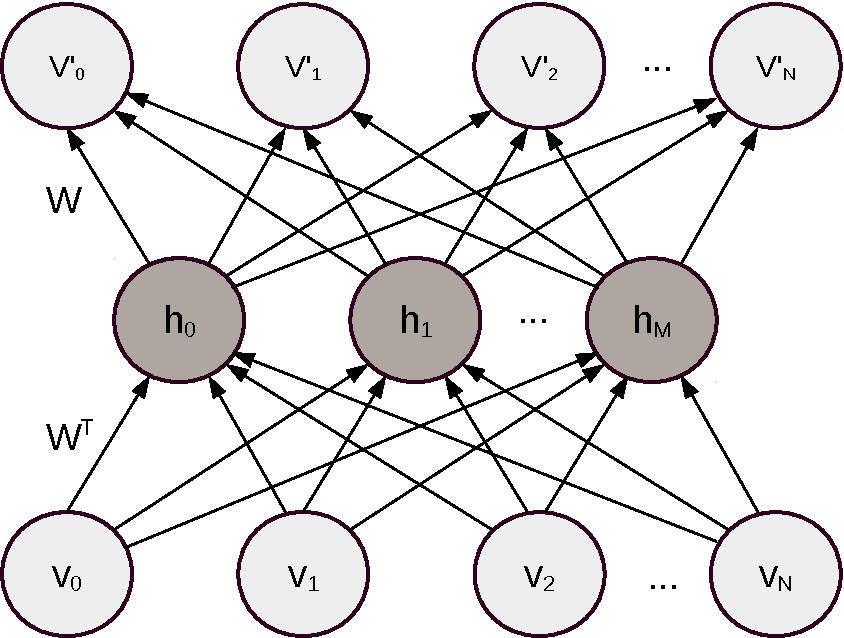
\includegraphics[width=0.4\textwidth]{AE}
	\caption{A typical Autoencoder structure.}
	\label{fig:AE}
\end{figure}

%TODO why tied weights are good
Notice that the connections used in the example are tied weights.
\begin{equation}
h_j=\sigma(\sum_i v_i w^T_{ij})
\end{equation}
\begin{equation}
v'_j=\sigma(\sum_i h_i w_{ij})
\end{equation}

Training an autoencoder is not different from backpropagation (BP) on an Multi-Layer Perceptrons(MLP).
The objective of training is to minimise the prediction error of an MLP, which measured as a loss function.
Accordingly, the loss function of an autoencoder can be described as:
\begin{equation}
L=\sum_{k=1}^{K}\|\mathbf{v}_{k}-\mathbf{v'}_{k}\|=\frac{1}{2}\sum_{k=1}^{K}(\mathbf{v}_{k}-\mathbf{v'}_{k})^{2}
\end{equation}
where k indicates the index of the training data $\mathbf{v}$, and each data vector $\mathbf{v}=\{v_0, v_1,...,v_N\}$ and its reconstruction $\mathbf{v'}=\{v'_0, v'_1,...,v'_N\}$ have N dimensions. 

%TODO rewording
Backpropagation, an abbreviation for "backward propagation of errors", is a common method of training artificial neural networks used in conjunction with an optimization method such as gradient descent.
The method calculates the gradient of a loss function with respect to all the weights in the network.
The gradient is fed to the optimisation method which in turn uses it to update the weights, in an attempt to minimize the loss function:
\begin{equation}
\Delta W \propto -\frac{\partial L}{\partial W}.
\end{equation}

Applying stochastic gradient descent (SGD), the true gradient of the weight matrix, $\Delta W$, is approximated by a gradient at a single example with iterations.
The reconstruction error $E_k$ of an input vector $\mathbf{v}_k$ is as given:
\begin{equation}
%	\begin{align*}
E_k = \frac{1}{2}(\mathbf{v}_k - \mathbf{v'}_k)^2,
%	\end{align*}
\end{equation}
and the gradient of the weight matrix is:
\begin{equation}
\Delta W \propto -\frac{\partial E_k}{\partial W}=-\eta \frac{\partial E_k}{\partial W},
\end{equation}
where $\eta$ is the learning rate.

Since we use tied weights in the network, the weight tuning only needs to apply in the output layer.
\begin{equation}
\begin{aligned}
\Delta w_{ij} = -\eta \frac{\partial E_k}{\partial w_{ij}} &= -\eta \frac{\partial E_k}{\partial v'_j} \frac{\partial v'_j}{\partial net\_v'_j} \frac{\partial net\_v'_j}{\partial w_{ij}}, \textrm{ where} \\
\frac{\partial E_k}{\partial v'_j} &= \frac{\partial \frac{1}{2}(\mathbf{v}_k - \mathbf{v'}_k)^2}{\partial v'_j}= -(v_j - v'_j), \\
%	\frac{\partial v'_j}{\partial net\_v'_j} &= \begin{cases} 1, v'_j>0\\0, v'_j<=0\\ \end{cases}, \textrm{using ReLU,}\\
\frac{\partial v'_j}{\partial net\_v'_j} &= 1, \textrm{using Identify function,}\\
\frac{\partial net\_v'_j}{\partial w_{ij}} &= \frac{\partial h_i w_{ij}}{\partial w_{ij}} = h_i.
\end{aligned}
\end{equation}
Thus, the weight gradient is calculated as:
\begin{equation}
\Delta w_{ij} = \eta h_i(v_j - v'_j) = \eta (h_i v_j - h_i v'_j)
\end{equation}
For RBMs:
\begin{equation}
\Delta w_{ij} = \eta (h_i v_j - h'_i v'_j)
\end{equation}
Energy of an Antoencoder:
\begin{equation}
H = \sum_{i}\sum_{j} v_i w_{ij} h_j.
\end{equation}
Examples of using an autoencoder with 10 input neurons and 10 hidden neurons: reconstruction the input data $\mathbf{v}$ where I) $v_i = 1$, II) $v_i = i/10$.
\begin{figure}
	\subfloat[Weights of Exp1]{
		\centering
		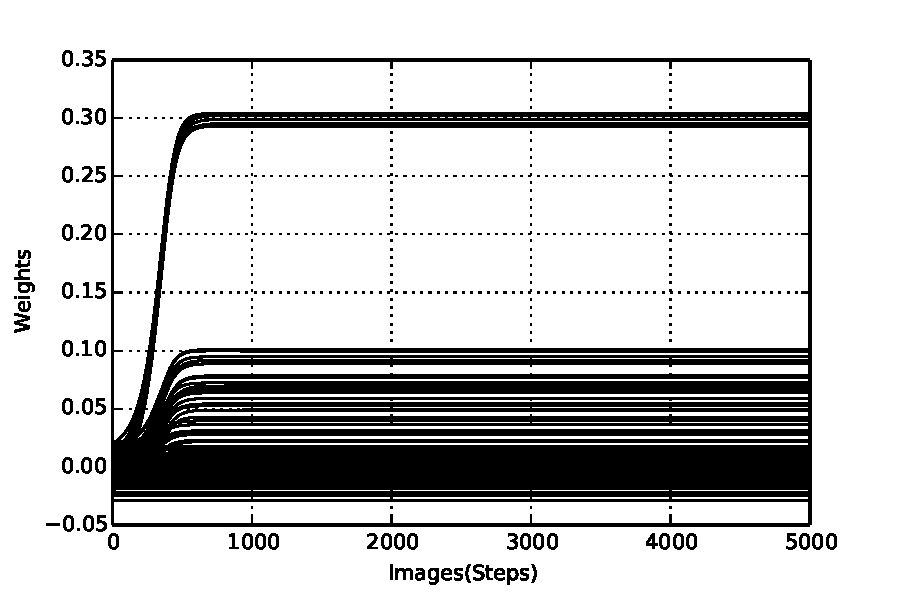
\includegraphics[width=0.25\textwidth]{exp1_weights_non}
	}
	\subfloat[Weights of Exp2]{
		\centering
		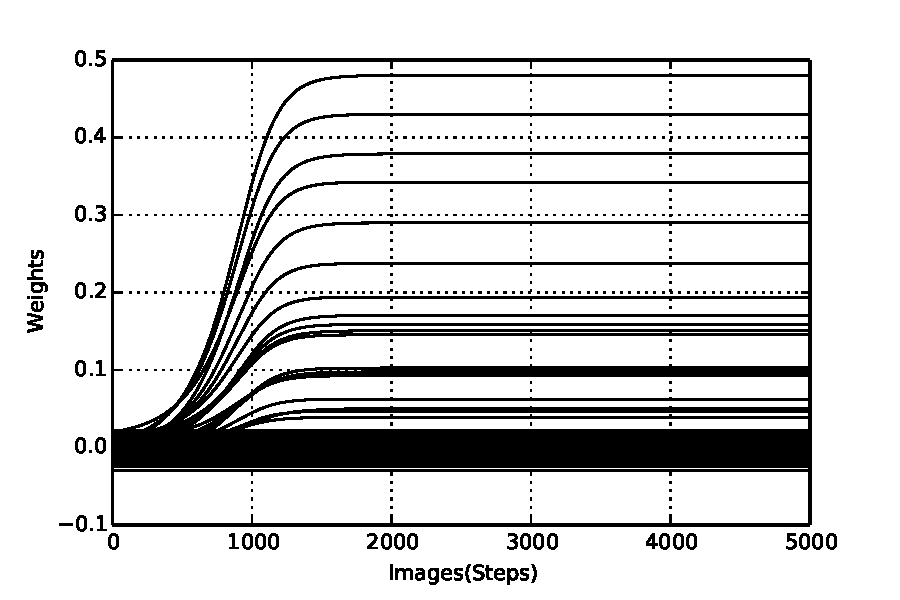
\includegraphics[width=0.25\textwidth]{exp2_weights_non}
	}\\
	\subfloat[Reconstruction of visible units in Exp1]{
		\centering
		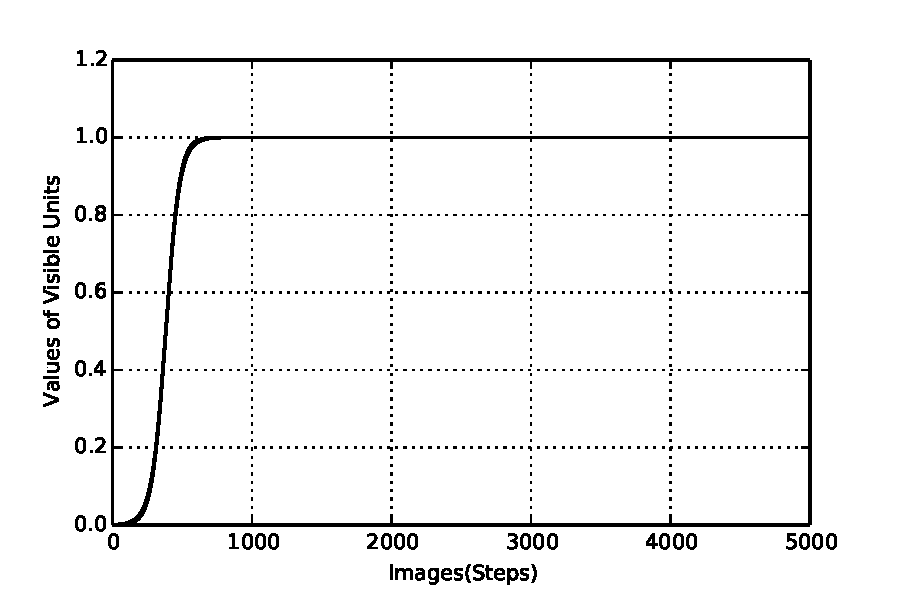
\includegraphics[width=0.25\textwidth]{exp1_recon_non}
	}
	\subfloat[Reconstruction of visible units in Exp2]{
		\centering
		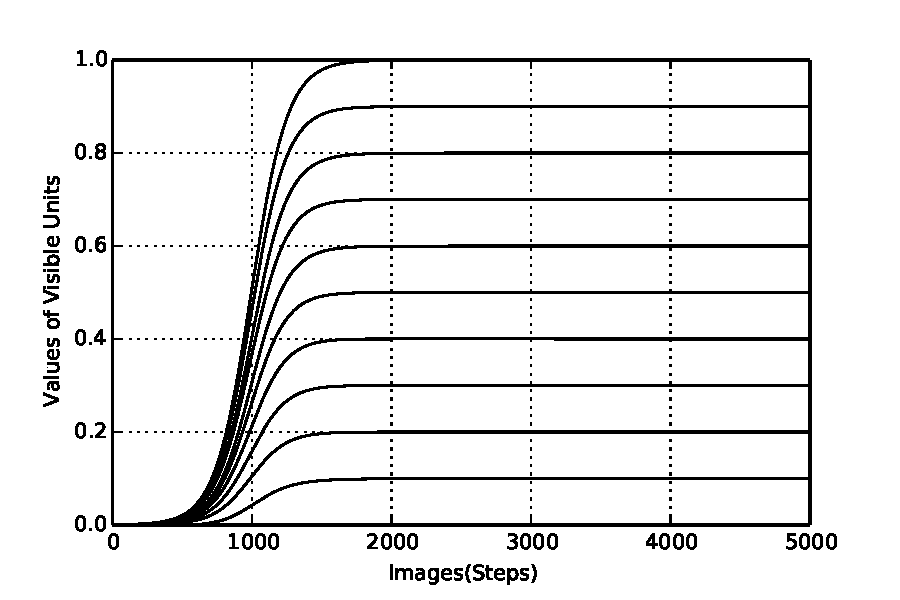
\includegraphics[width=0.25\textwidth]{exp2_recon_non}
	}\\
	\subfloat[Output of hidden units in Exp1]{
		\centering
		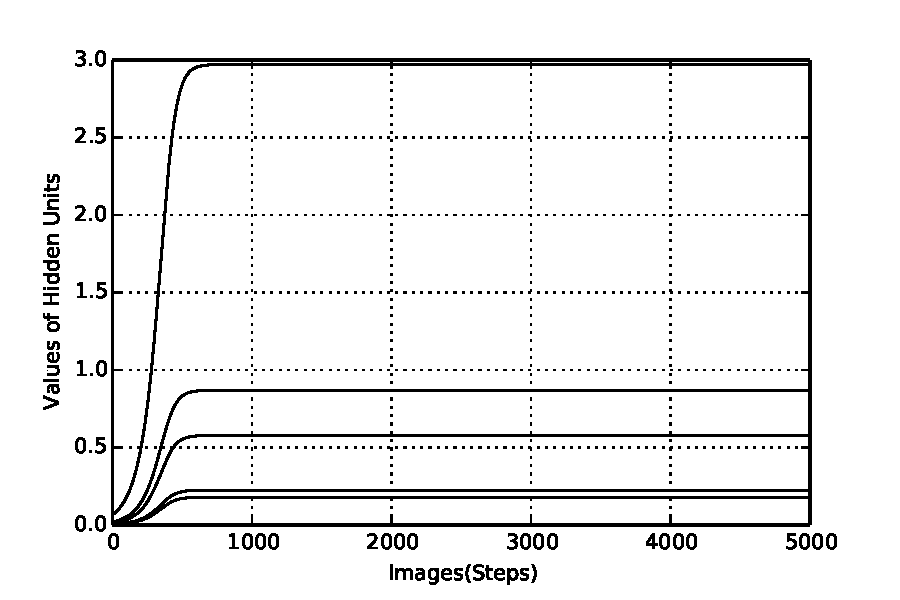
\includegraphics[width=0.25\textwidth]{exp1_hid_non}
	}
	\subfloat[Output of hidden units in Exp2]{
		\centering
		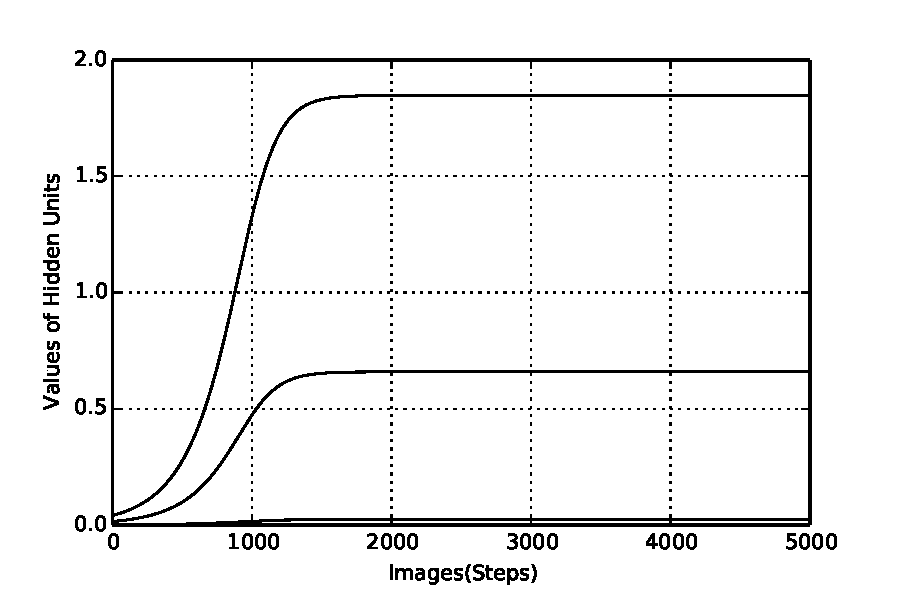
\includegraphics[width=0.25\textwidth]{exp2_hid_non}
	}
	\caption{Weights and outputs of visible and hidden units change during training of the reconstruction tests. 
		Experiments 1) 10 visible units fully connected to 10 hidden units with input data of all 1s; 2) same network fed with 10 values distribute linearly from 0.1 to 1.}
\end{figure}

\subsection{Training Spiking Autoencoders}
Rate-based learning of STDP (rSTDP) which is inspired by ReSuMe.\\
-Why it works stated in Maths.\\
\begin{equation}
\begin{aligned}
\overline{\Delta w_{ij}} &\propto \eta \lambda_{h_i}(\lambda_{v_j} - \lambda_{v'_j})\\
&=\eta'P_{h_i}P_{v_j}\tau_{w} \tau_{dur} - \eta'P_{h_i}P_{v'_j}\tau_{w} \tau_{dur}, \textrm{where,}\\
P_{s} &= \lambda_{s} \times 0.001~s = \frac{K s}{1000}\\
\eta' &= \frac{10^6}{K^2 \tau_{w} \tau_{dur}} \eta
\end{aligned}
\end{equation}

-Figure to plot
\begin{figure}
	\centering
	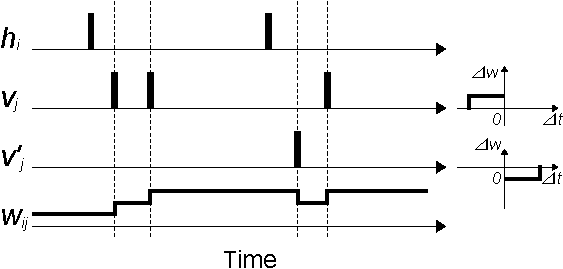
\includegraphics[width=0.5\textwidth]{rSTDP}
	\caption{How rSTDP works in training AutoEncoders.}
	\label{fig:rSTDP}
\end{figure}


Experiments
\begin{figure}
	\subfloat[Weights of Exp1]{
		\centering
		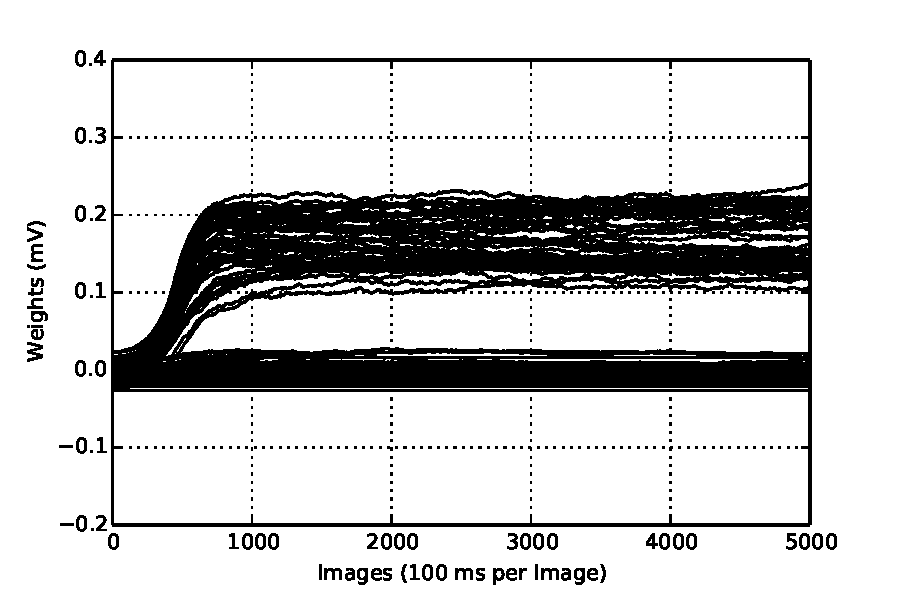
\includegraphics[width=0.25\textwidth]{exp1_weights_s}
	}
	\subfloat[Weights of Exp2]{
		\centering
		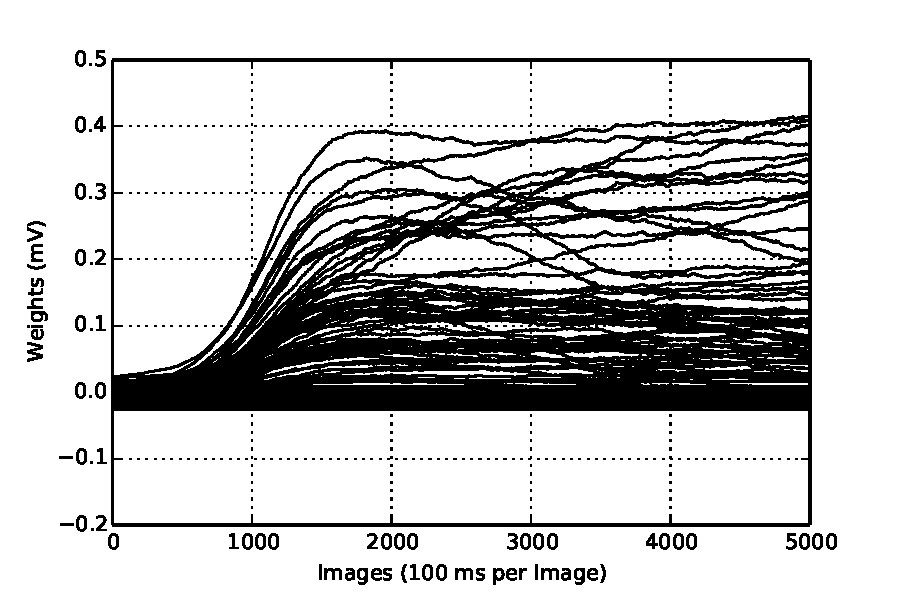
\includegraphics[width=0.25\textwidth]{exp2_weights_s}
	}\\
	\subfloat[Reconstruction of visible units in Exp1]{
		\centering
		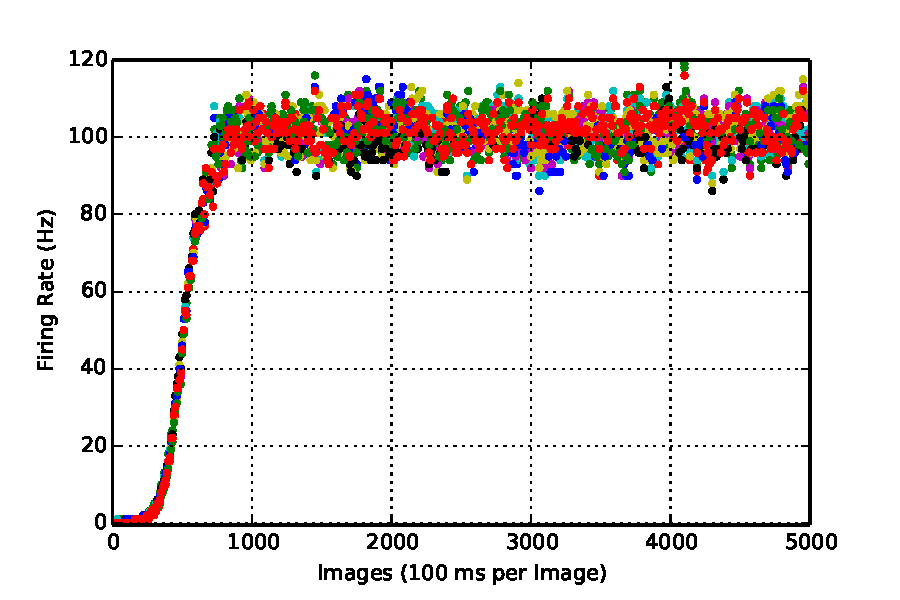
\includegraphics[width=0.25\textwidth]{exp1_recon_s}
	}
	\subfloat[Reconstruction of visible units in Exp2]{
		\centering
		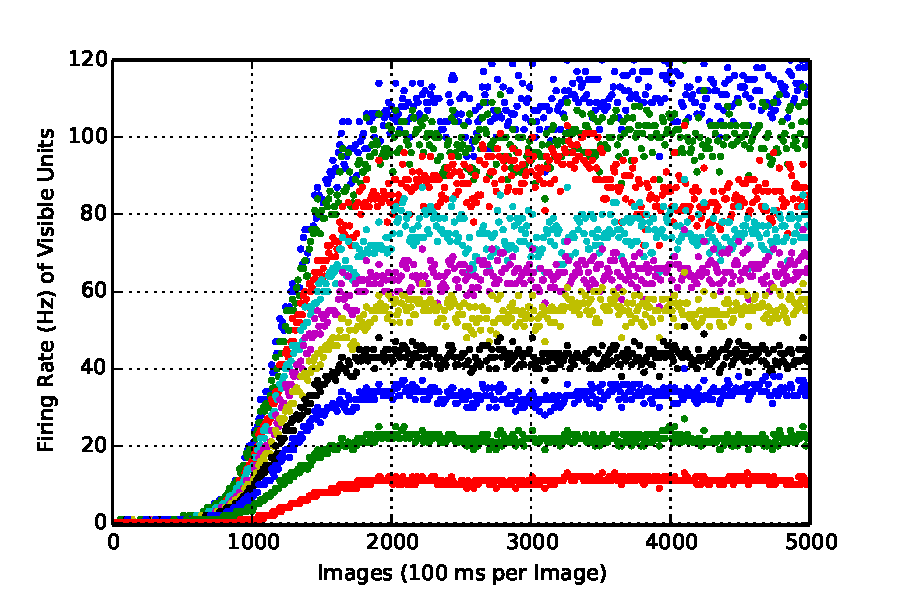
\includegraphics[width=0.25\textwidth]{exp2_recon_s}
	}\\
	\subfloat[Reconstruction of visible units in Exp1]{
		\centering
		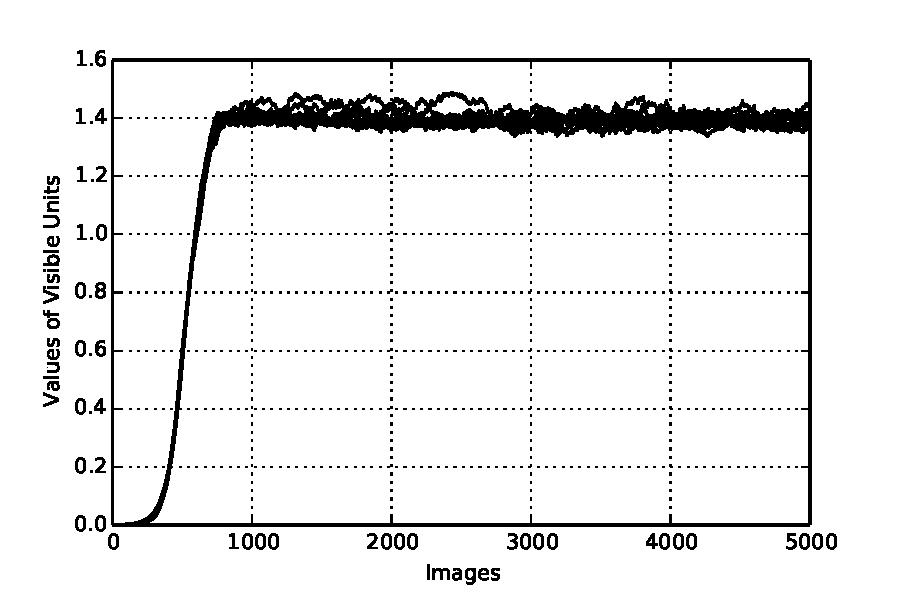
\includegraphics[width=0.25\textwidth]{exp1_recon_nons}
	}
	\subfloat[Reconstruction of visible units in Exp2]{
		\centering
		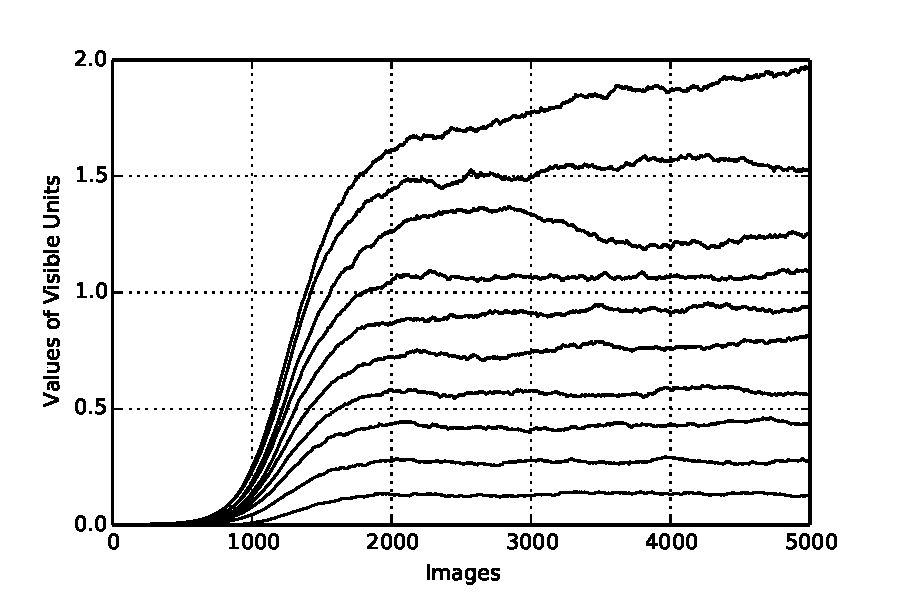
\includegraphics[width=0.25\textwidth]{exp2_recon_nons}
	}\\
	\subfloat[Reconstruction of visible units in Exp1]{
		\centering
		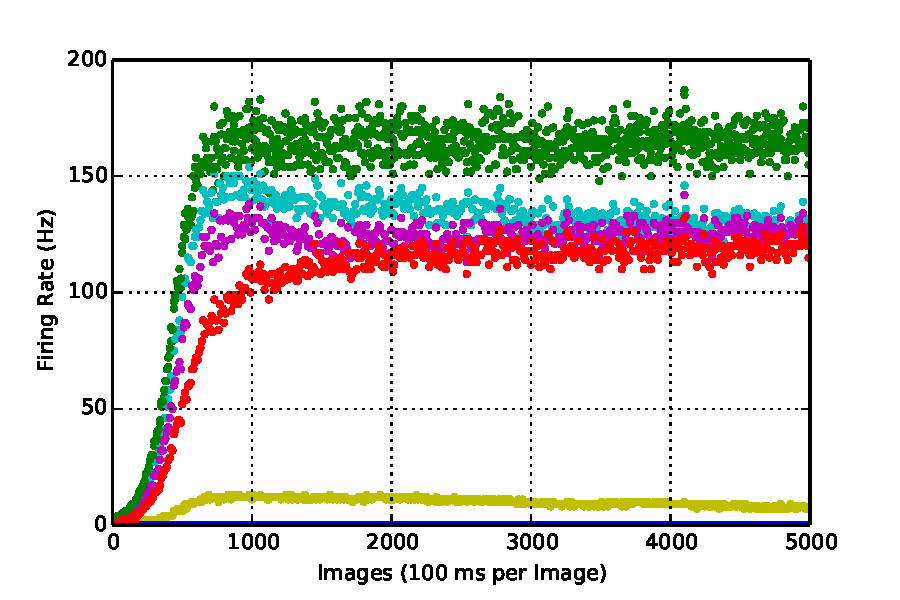
\includegraphics[width=0.25\textwidth]{exp1_hid_s}
	}
	\subfloat[Reconstruction of visible units in Exp2]{
		\centering
		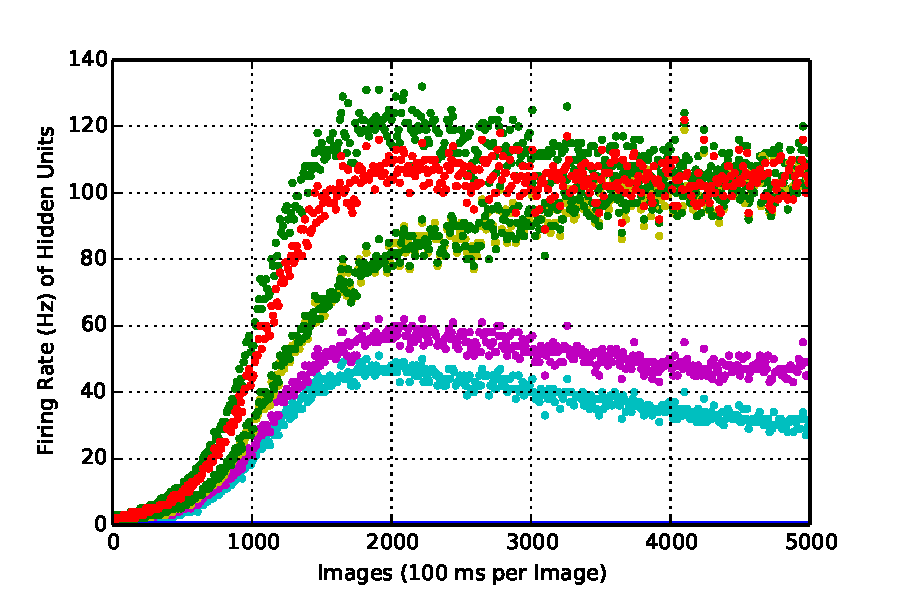
\includegraphics[width=0.25\textwidth]{exp2_hid_s}
	}\\
	\subfloat[Output of hidden units in Exp1]{
		\centering
		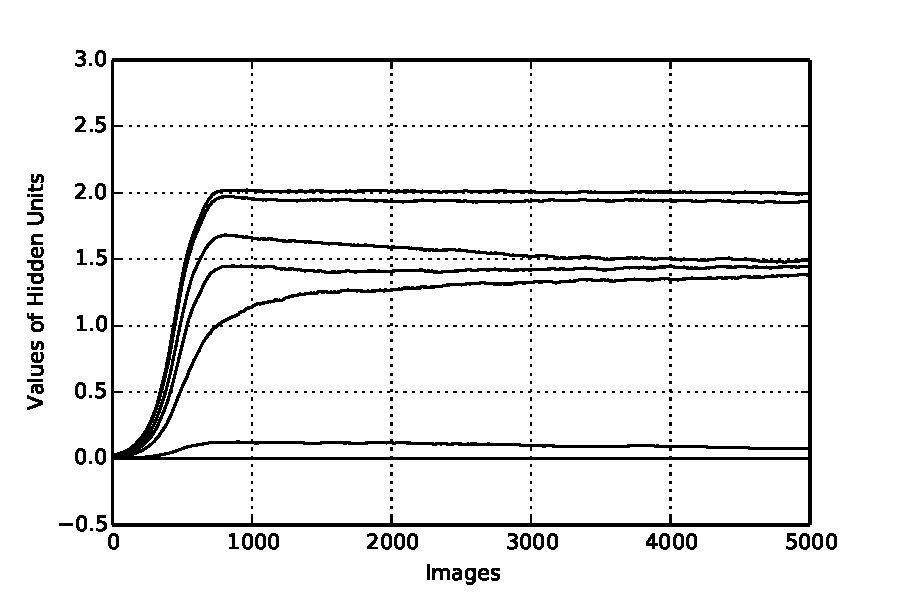
\includegraphics[width=0.25\textwidth]{exp1_hid_nons}
	}
	\subfloat[Output of hidden units in Exp2]{
		\centering
		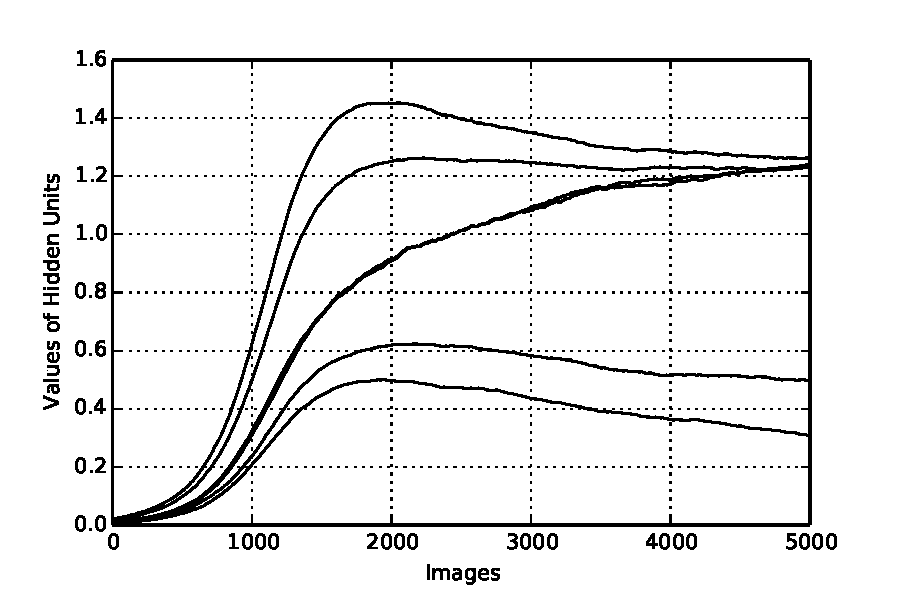
\includegraphics[width=0.25\textwidth]{exp2_hid_nons}
	}
	\caption{Weights and firing rates of visible and hidden units change during training of the reconstruction tests of spiking neurons. 
		Experiments 1) 10 visible units fully connected to 10 hidden units with Poisson spike trains of 100~Hz which lasted 100~ms; 2) same network fed with 10 Poisson spike trains of firing rate ranging from 10~Hz to 100~Hz.}
\end{figure}
\subsection{Problem}
Poisson noise make weights diverge.
Same Poisson data used in non-spiking tests.
\begin{figure}
	\subfloat[Weights of Exp1]{
		\centering
		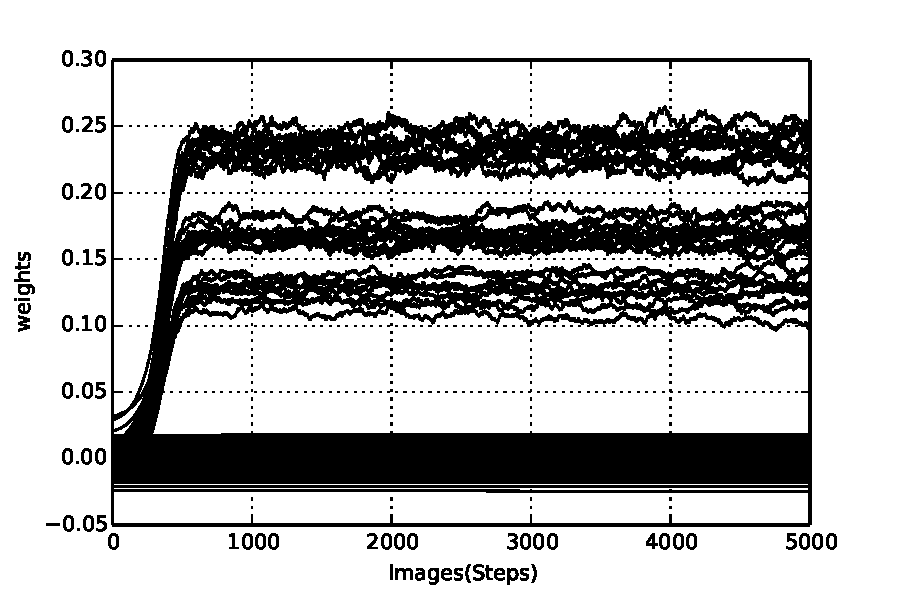
\includegraphics[width=0.25\textwidth]{exp1_weights_noisy}
	}
	\subfloat[Weights of Exp2]{
		\centering
		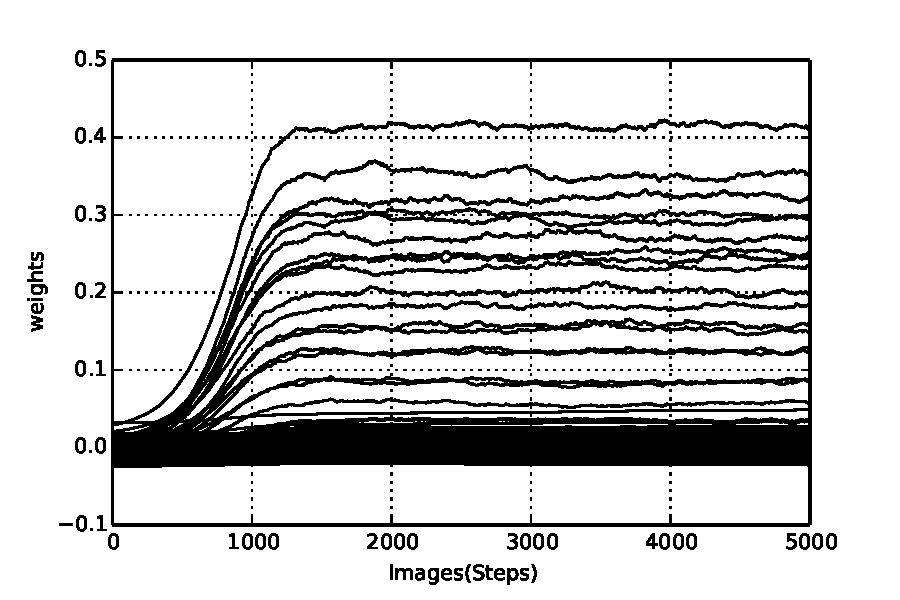
\includegraphics[width=0.25\textwidth]{exp2_weights_noisy}
	}\\
	\subfloat[Reconstruction of visible units in Exp1]{
		\centering
		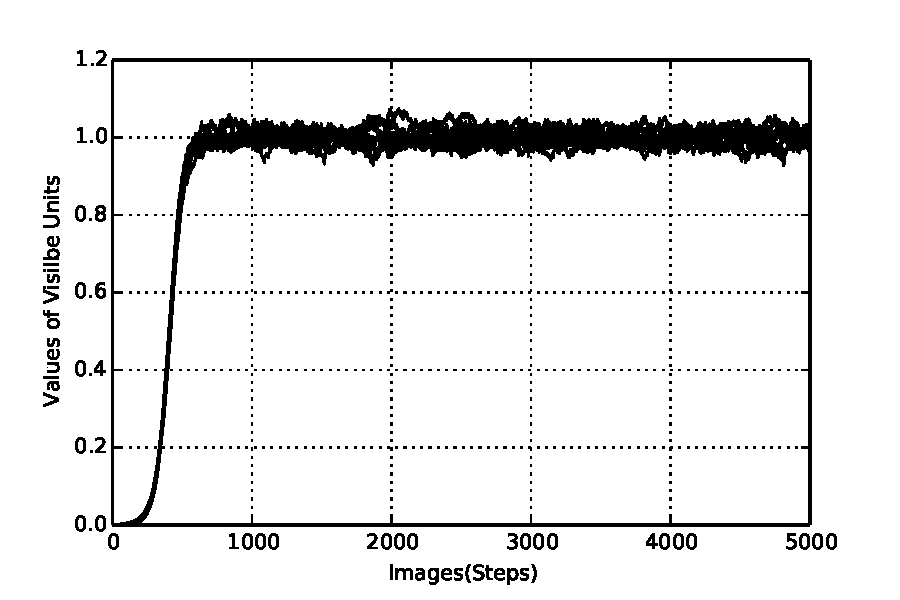
\includegraphics[width=0.25\textwidth]{exp1_recon_noisy}
	}
	\subfloat[Reconstruction of visible units in Exp2]{
		\centering
		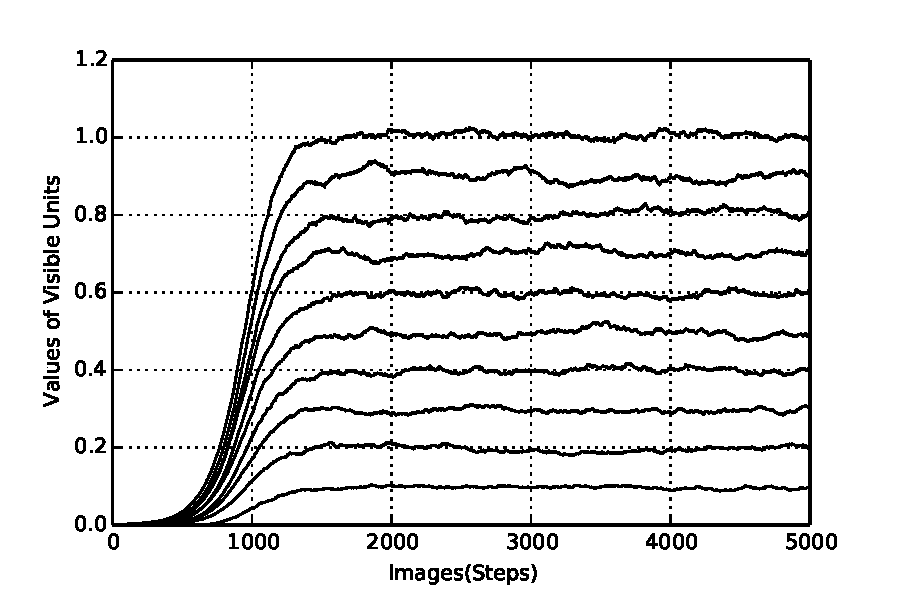
\includegraphics[width=0.25\textwidth]{exp2_recon_noisy}
	}\\
	\subfloat[Output of hidden units in Exp1]{
		\centering
		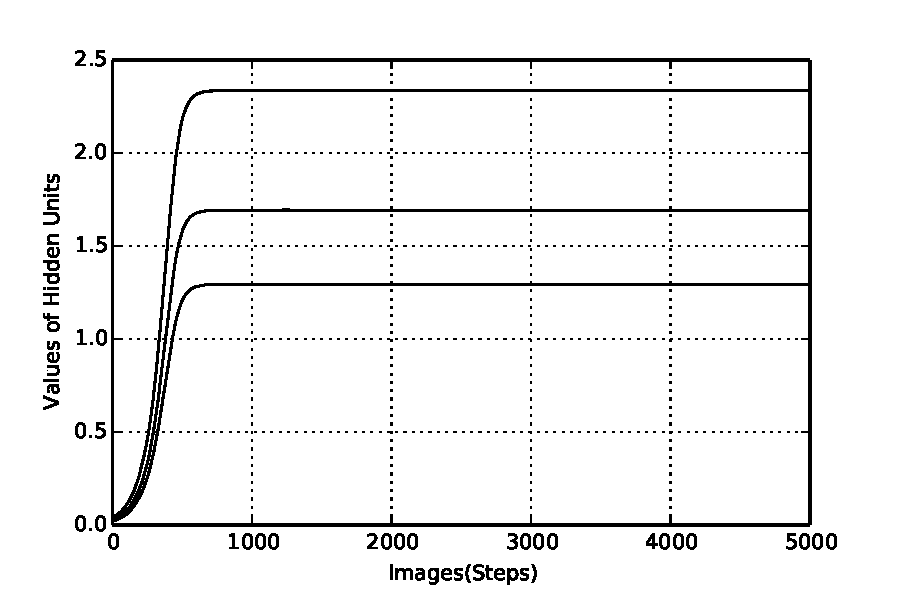
\includegraphics[width=0.25\textwidth]{exp1_hid_noisy}
	}
	\subfloat[Output of hidden units in Exp2]{
		\centering
		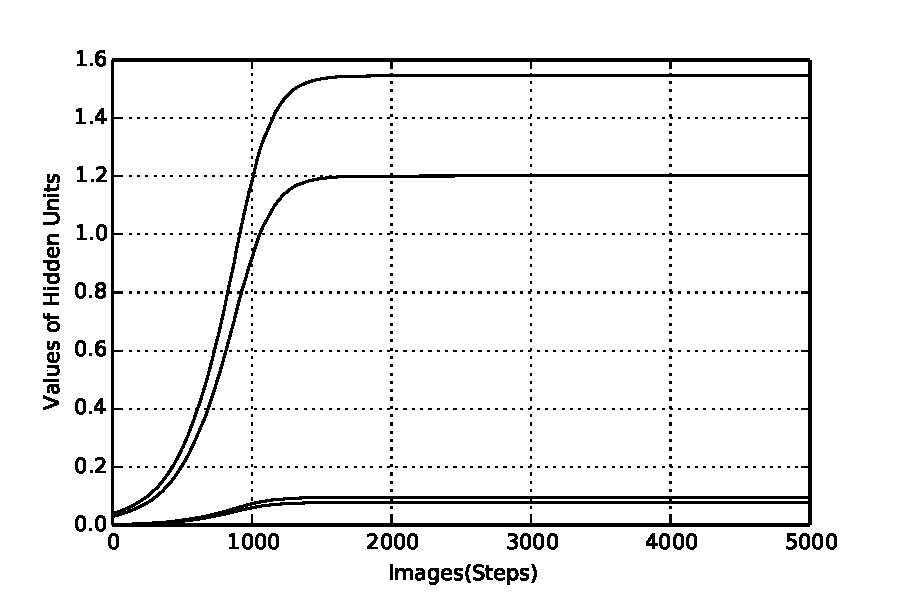
\includegraphics[width=0.25\textwidth]{exp2_hid_noisy}
	}
	\caption{Weights and outputs of visible and hidden units change during training fed with noisy inputs. 
		Experiments 1) 10 visible units fully connected to 10 hidden units with noisy input data of all 1s; 2) same network fed with noisy values distribute linearly from 0.1 to 1.}
\end{figure}

Decay learning rate.
\begin{figure}
	\subfloat[Weights of Exp1]{
		\centering
		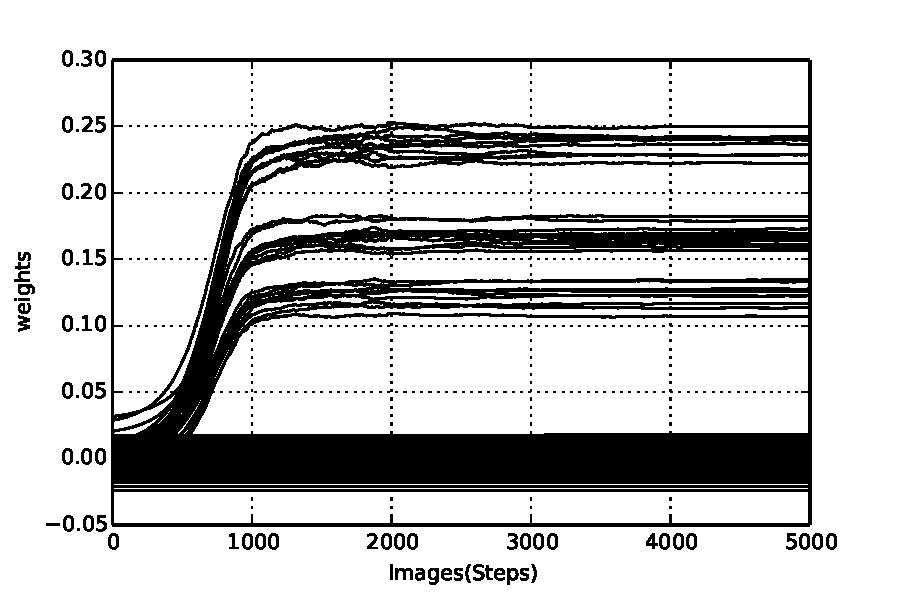
\includegraphics[width=0.25\textwidth]{exp1_weights_noisy_decay}
	}
	\subfloat[Weights of Exp2]{
		\centering
		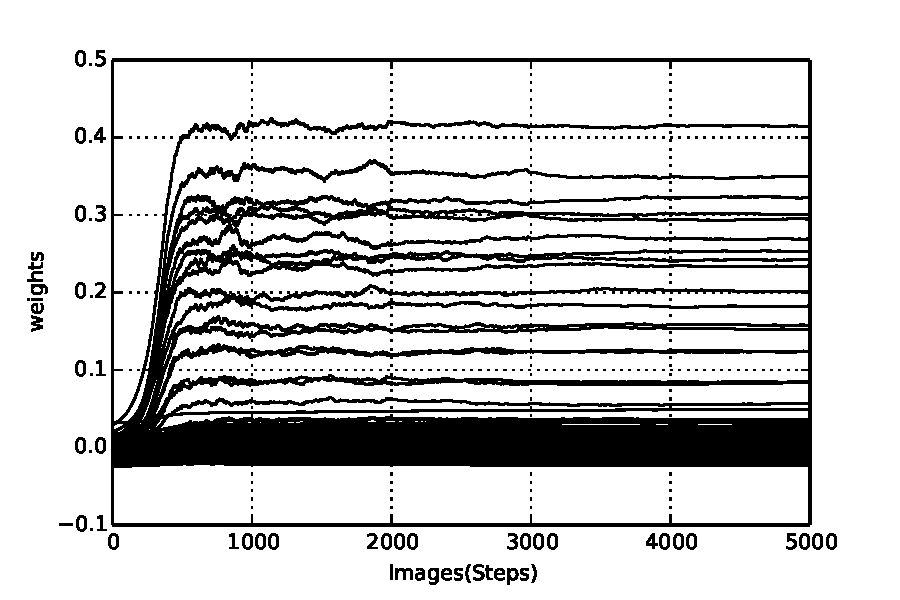
\includegraphics[width=0.25\textwidth]{exp2_weights_noisy_decay}
	}\\
	\subfloat[Reconstruction of visible units in Exp1]{
		\centering
		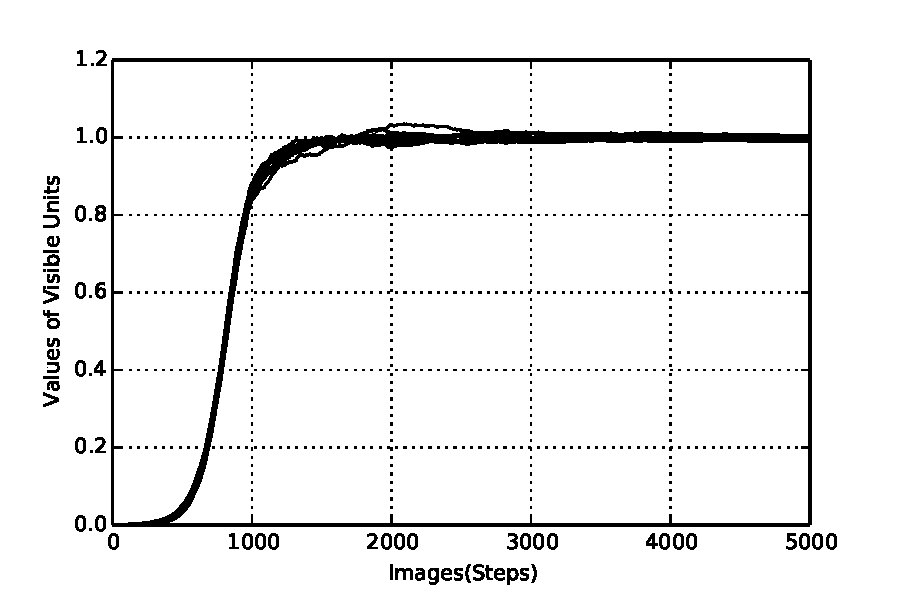
\includegraphics[width=0.25\textwidth]{exp1_recon_noisy_decay}
	}
	\subfloat[Reconstruction of visible units in Exp2]{
		\centering
		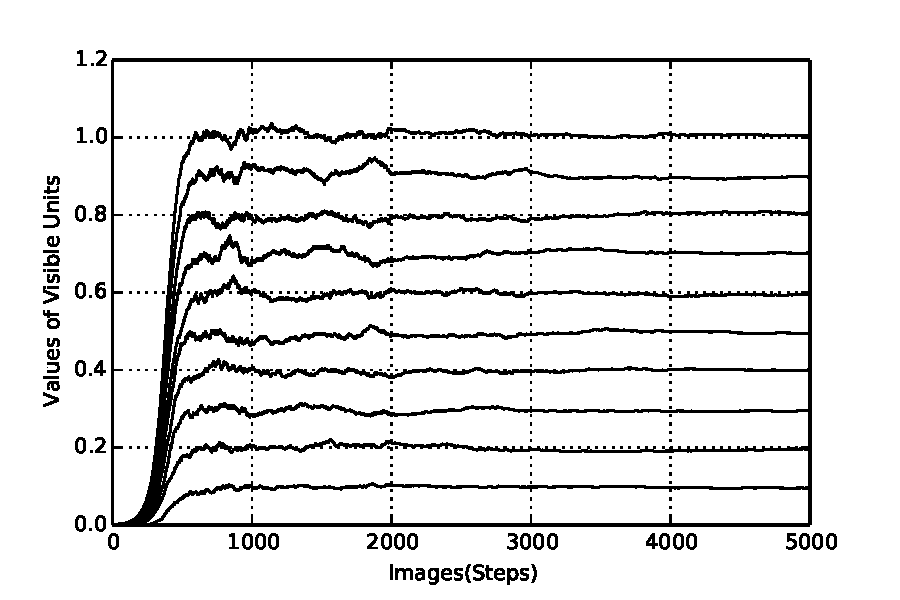
\includegraphics[width=0.25\textwidth]{exp2_recon_noisy_decay}
	}\\
	\subfloat[Output of hidden units in Exp1]{
		\centering
		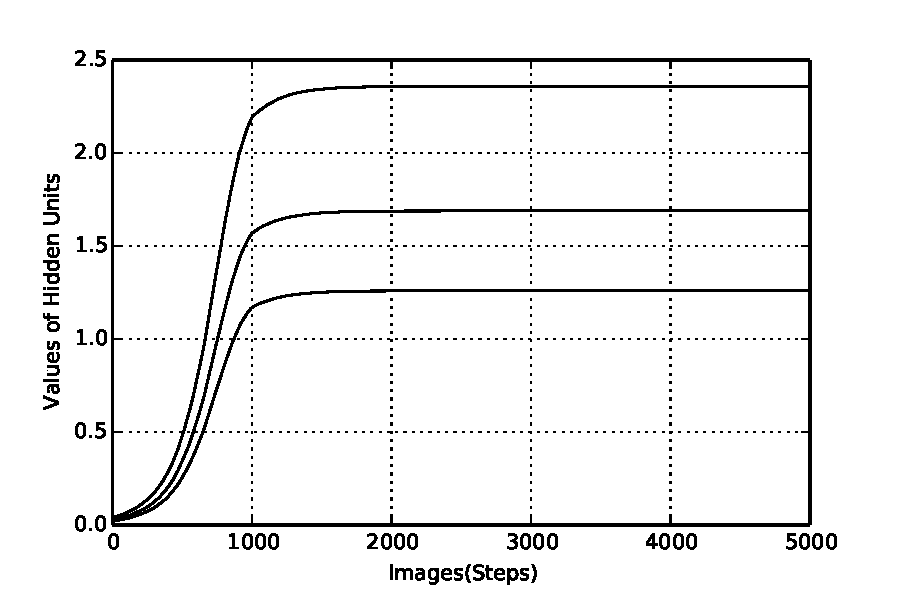
\includegraphics[width=0.25\textwidth]{exp1_hid_noisy_decay}
	}
	\subfloat[Output of hidden units in Exp2]{
		\centering
		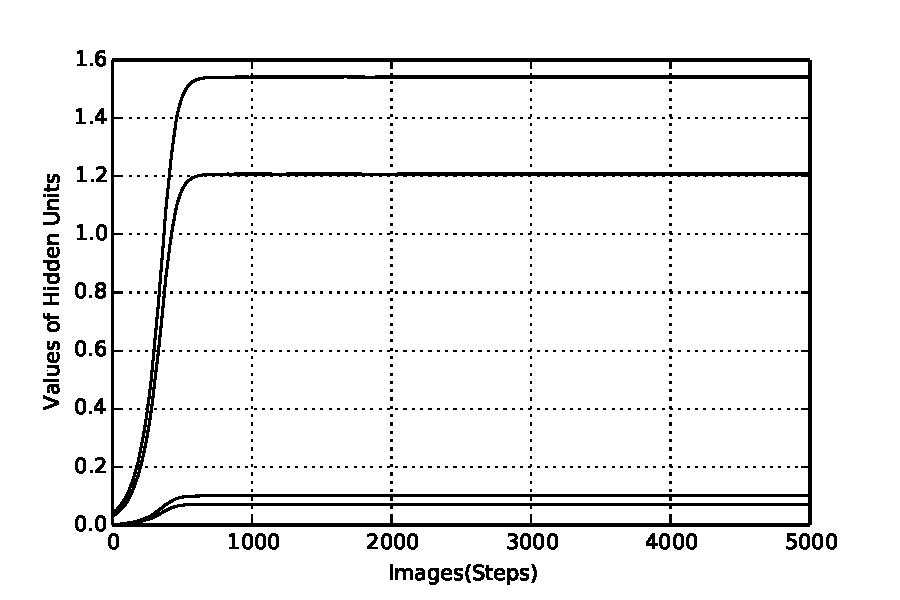
\includegraphics[width=0.25\textwidth]{exp2_hid_noisy_decay}
	}
	\caption{Weights and outputs of visible and hidden units change during training using decayed learning rate. 
		Experiments 1) 10 visible units fully connected to 10 hidden units with noisy input data of all 1s; 2) same network fed with noisy values distribute linearly from 0.1 to 1.}
\end{figure}

Decay learning rate in SNN.
\begin{figure}
	\subfloat[Weights of Exp1]{
		\centering
		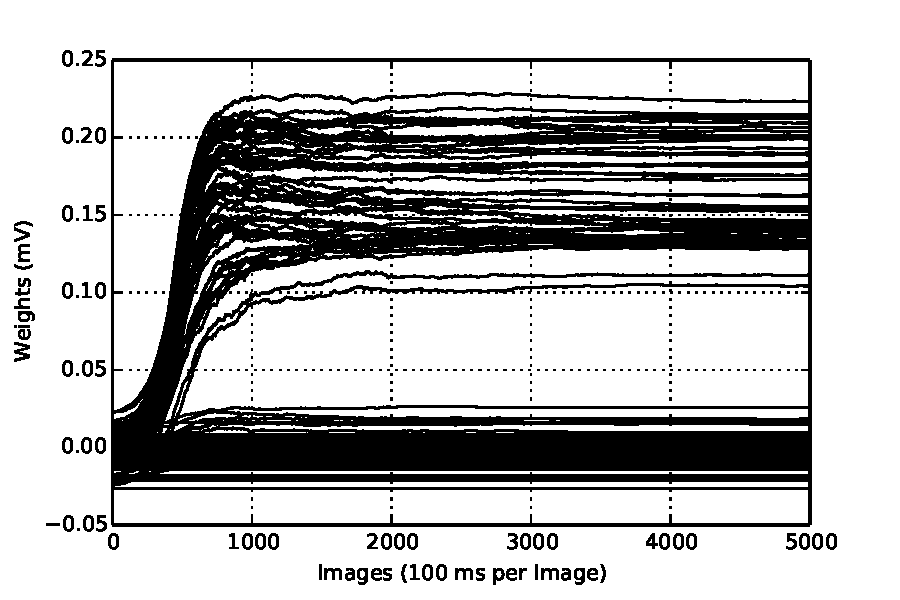
\includegraphics[width=0.25\textwidth]{exp1_weights_s_decay}
	}
	\subfloat[Weights of Exp2]{
		\centering
		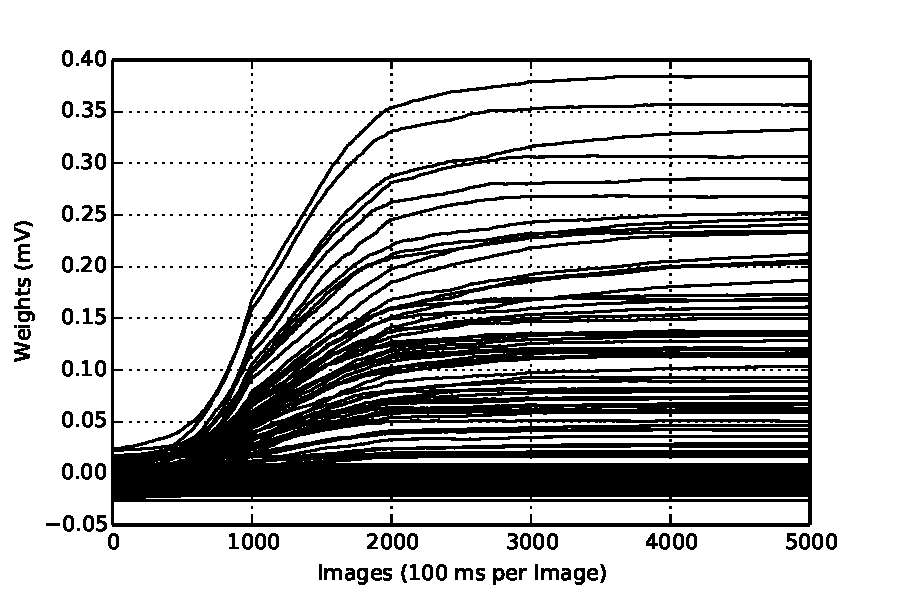
\includegraphics[width=0.25\textwidth]{exp2_weights_s_decay}
	}\\
	\subfloat[Reconstruction of visible units in Exp1]{
		\centering
		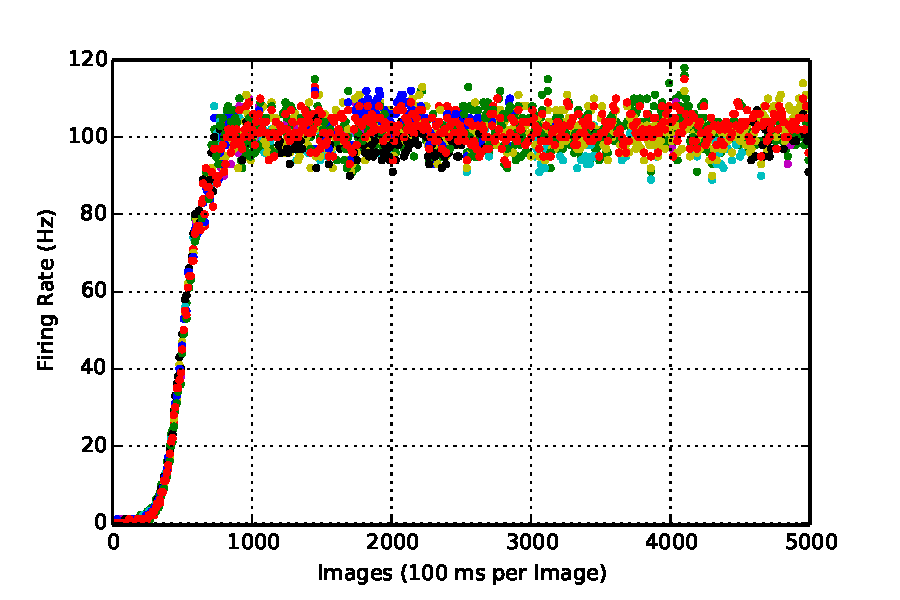
\includegraphics[width=0.25\textwidth]{exp1_recon_s_decay}
	}
	\subfloat[Reconstruction of visible units in Exp2]{
		\centering
		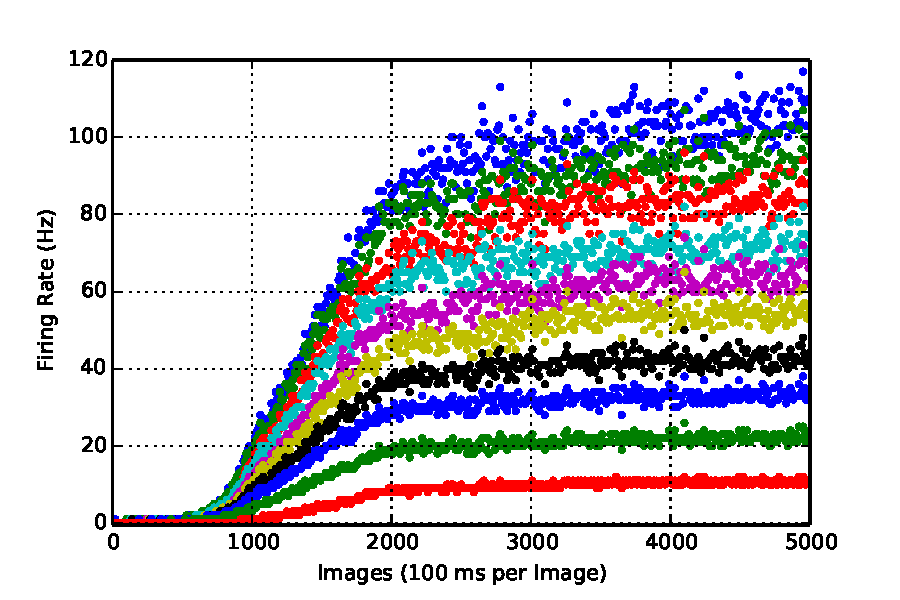
\includegraphics[width=0.25\textwidth]{exp2_recon_s_decay}
	}\\
	\subfloat[Reconstruction of visible units in Exp1]{
		\centering
		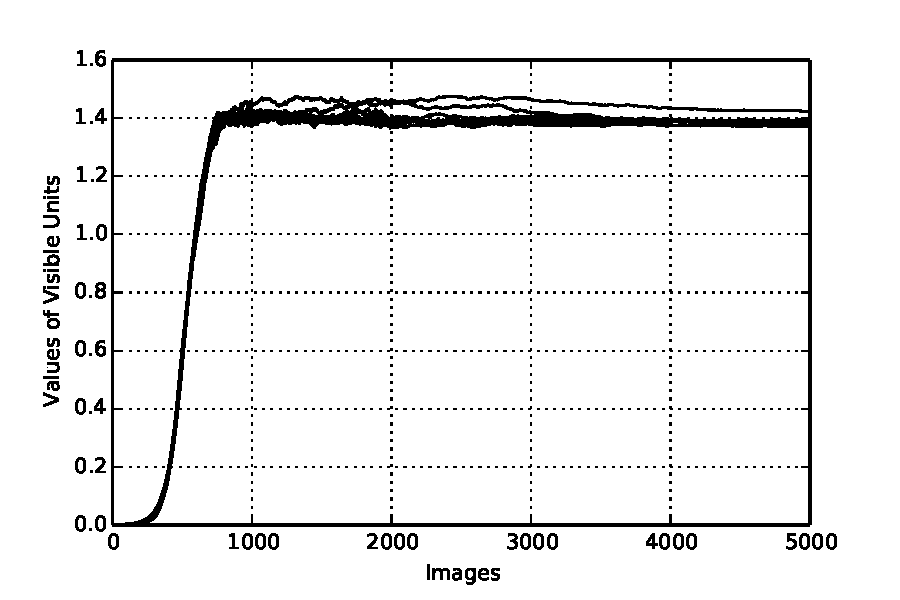
\includegraphics[width=0.25\textwidth]{exp1_recon_nons_decay}
	}
	\subfloat[Reconstruction of visible units in Exp2]{
		\centering
		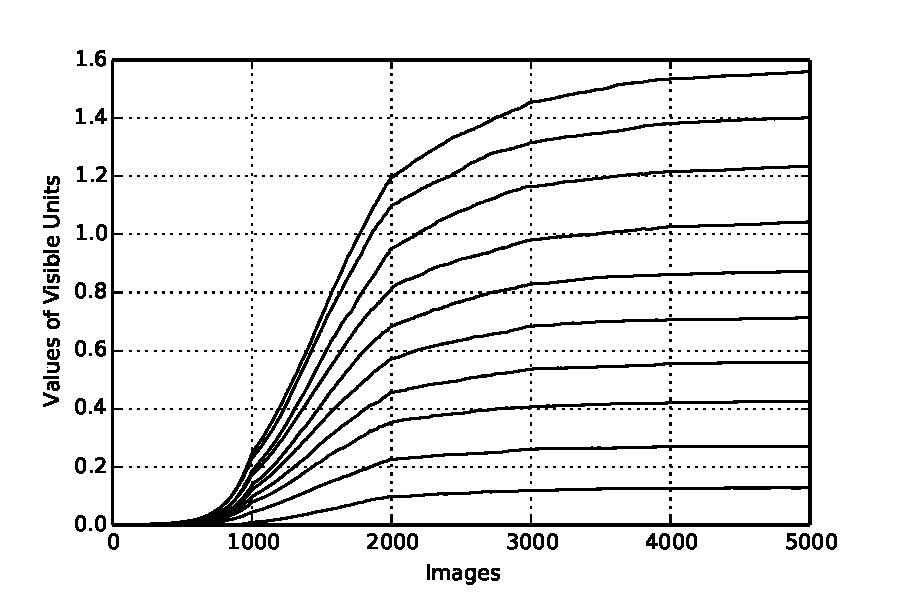
\includegraphics[width=0.25\textwidth]{exp2_recon_nons_decay}
	}\\
	\subfloat[Reconstruction of visible units in Exp1]{
		\centering
		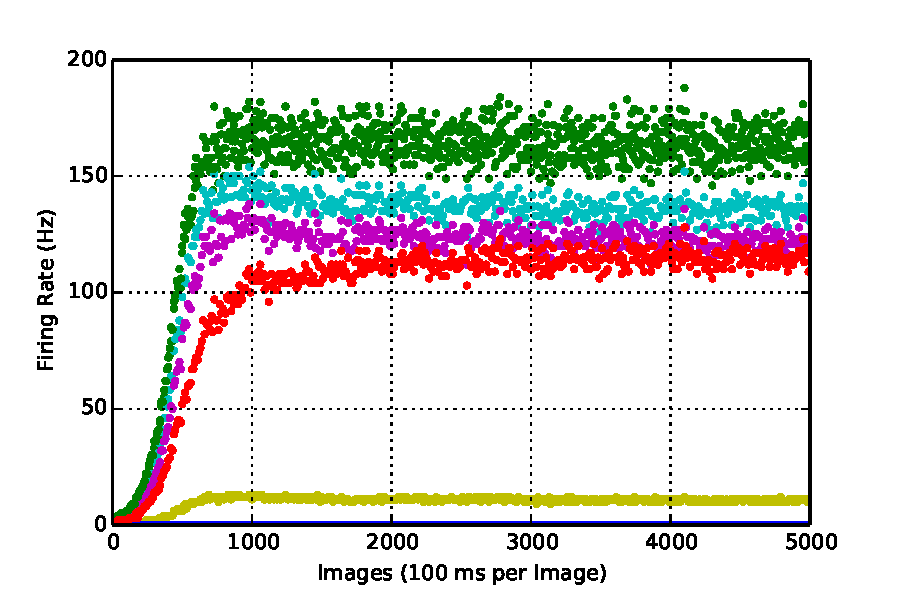
\includegraphics[width=0.25\textwidth]{exp1_hid_s_decay}
	}
	\subfloat[Reconstruction of visible units in Exp2]{
		\centering
		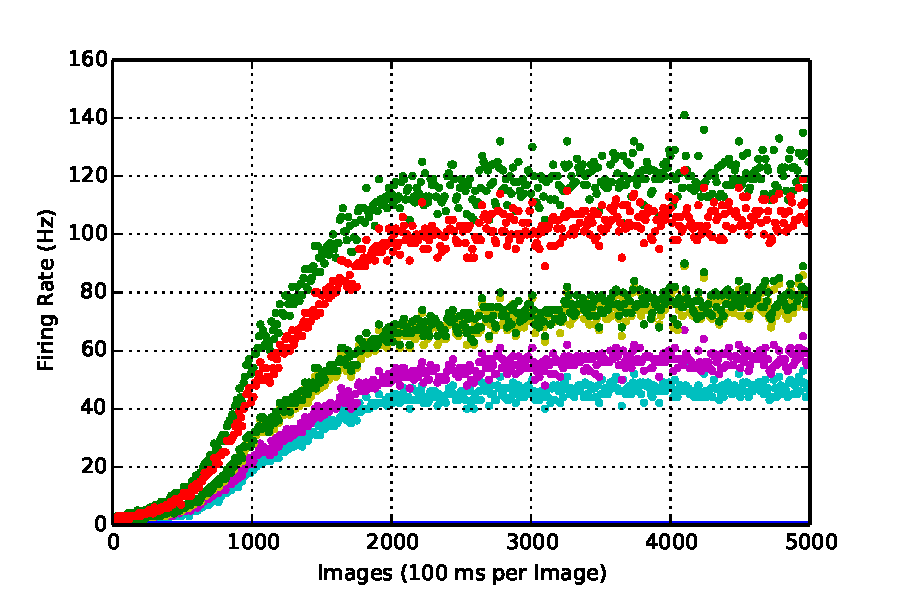
\includegraphics[width=0.25\textwidth]{exp2_hid_s_decay}
	}\\
	\subfloat[Output of hidden units in Exp1]{
		\centering
		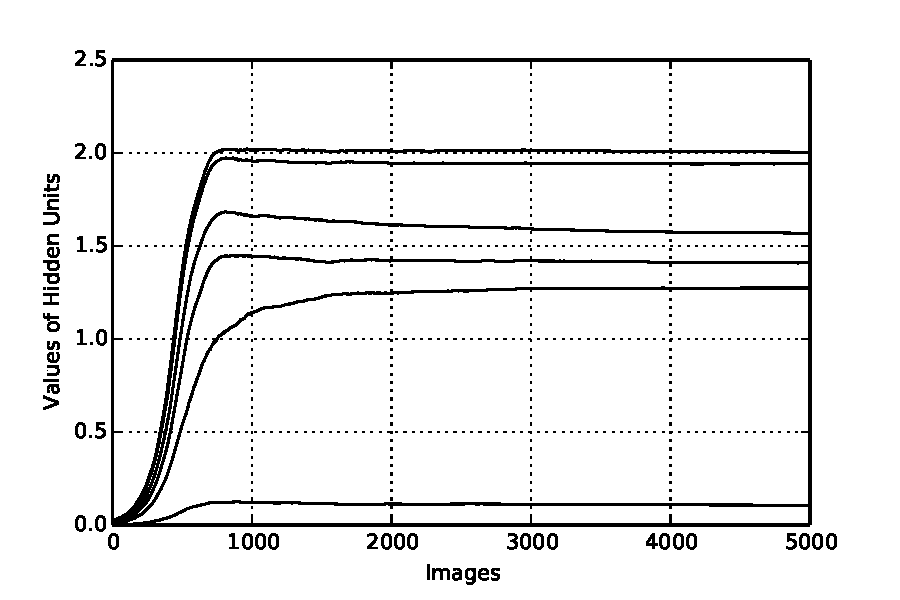
\includegraphics[width=0.25\textwidth]{exp1_hid_nons_decay}
	}
	\subfloat[Output of hidden units in Exp2]{
		\centering
		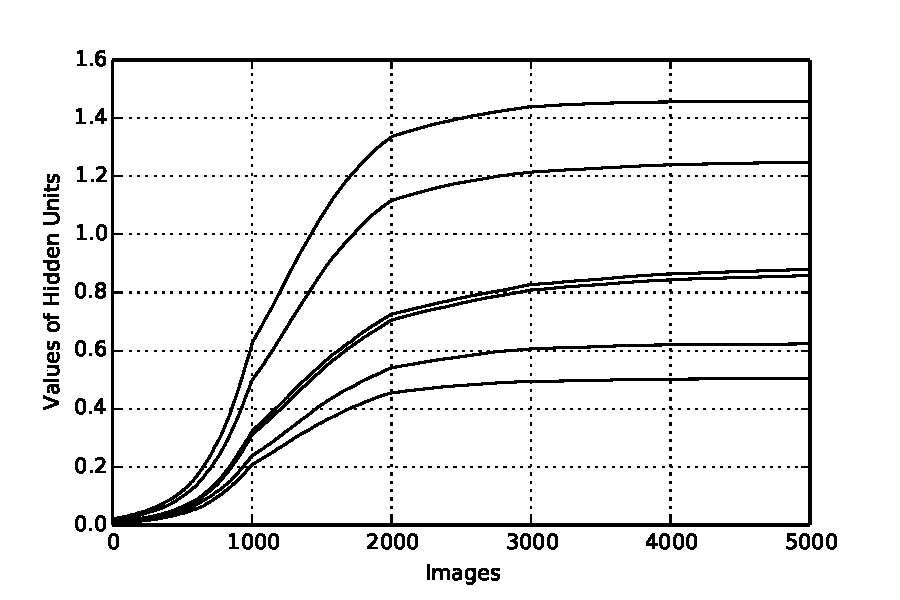
\includegraphics[width=0.25\textwidth]{exp2_hid_nons_decay}
	}
	\caption{Weights and firing rates of visible and hidden units change during training of the reconstruction tests of spiking neurons. 
		Experiments 1) 10 visible units fully connected to 10 hidden units with Poisson spike trains of 100~Hz which lasted 100~ms; 2) same network fed with 10 Poisson spike trains of firing rate ranging from 10~Hz to 100~Hz.}
\end{figure}
\section{Results}
Autoencoders work as recognition.
\begin{figure}
	\centering
	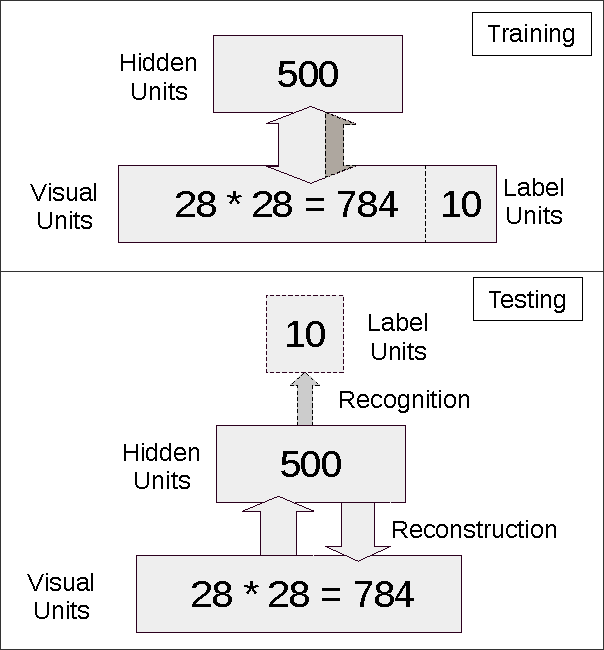
\includegraphics[width=0.4\textwidth]{mnist}
	\caption{One layer of Autoencoders work as a digit recogniser.}
	\label{fig:mnist}		
\end{figure}
\subsection{Trained weights}
AE automatically extracts features.
\begin{figure}
	\subfloat[Trained with 1000 Images]{
		\centering
		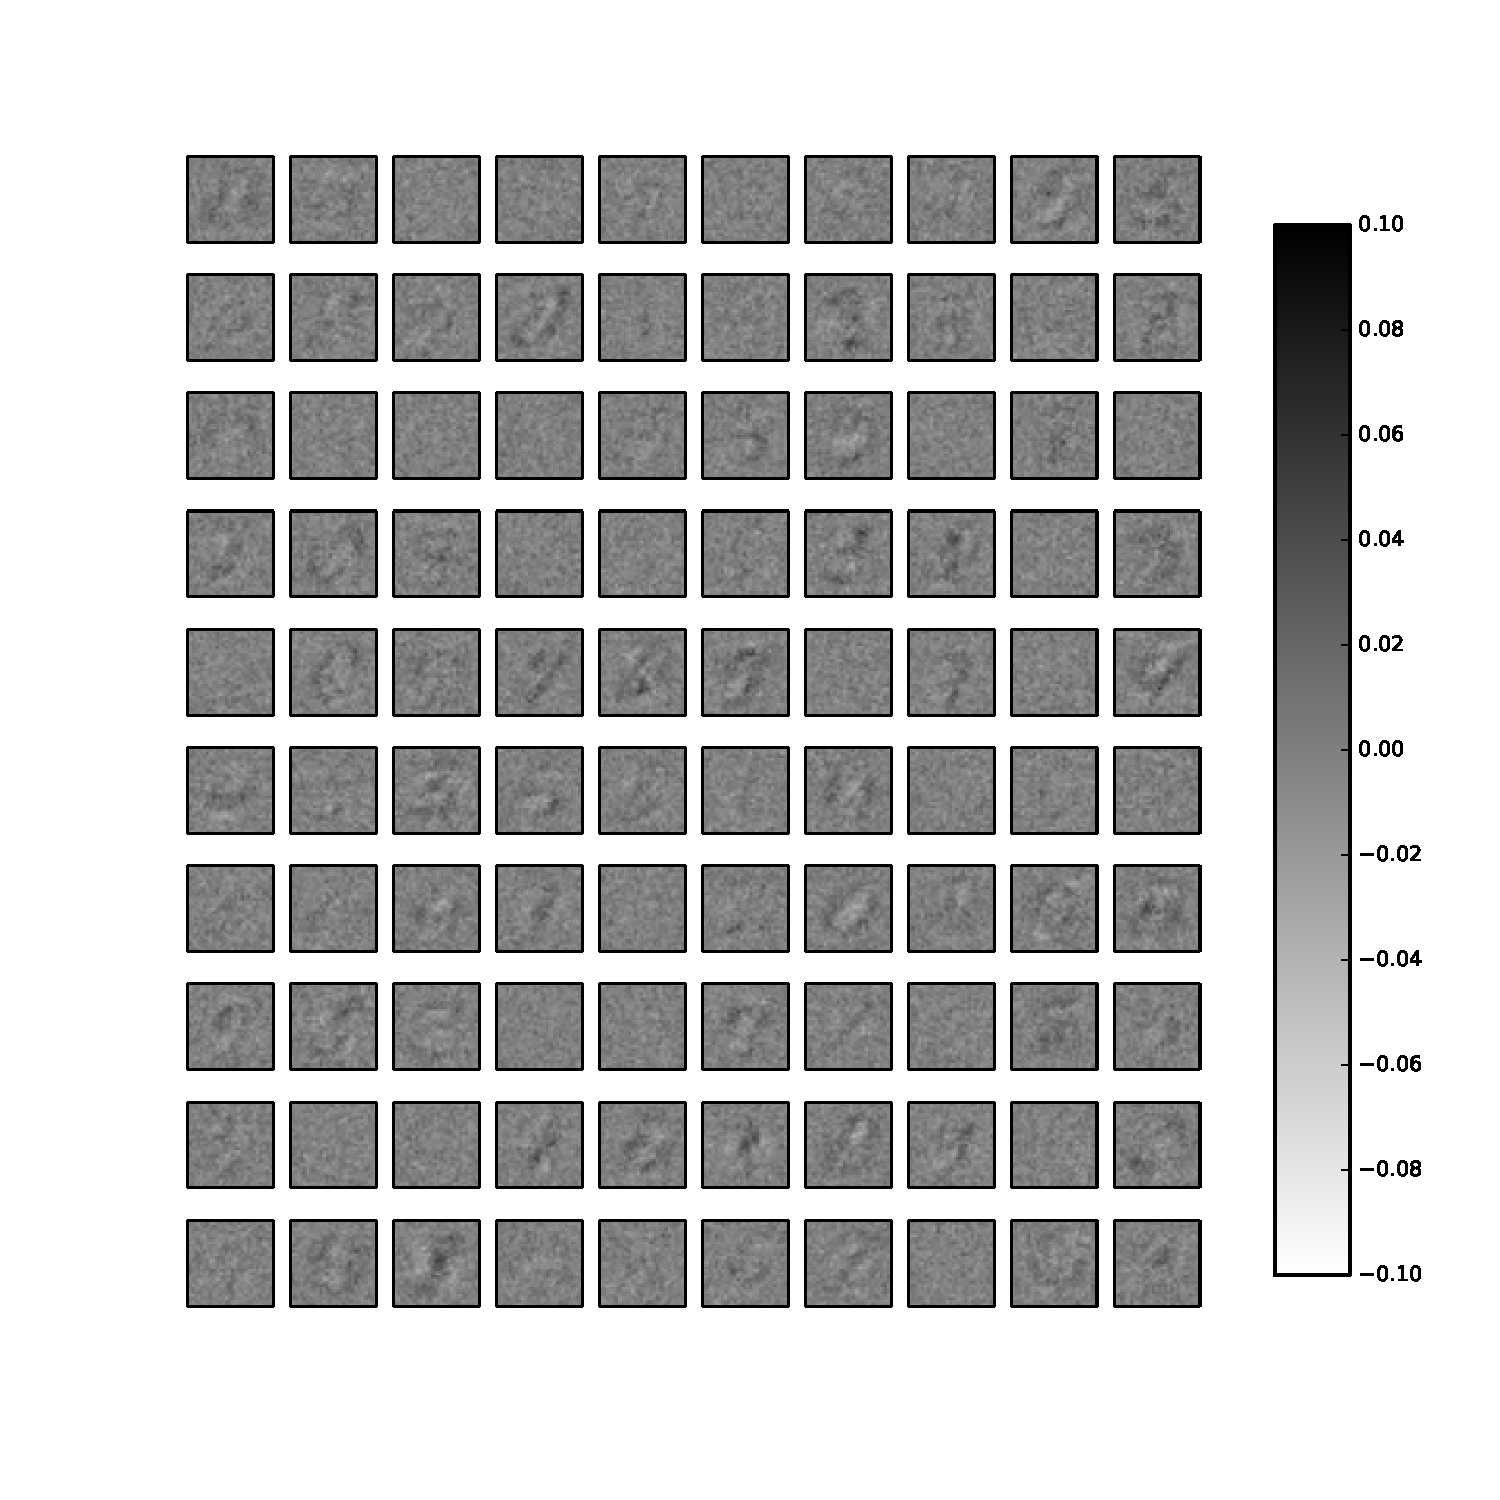
\includegraphics[width=0.5\textwidth]{weights_e0_1000}
	}\\
	\subfloat[Trained with 60000 Images]{
		\centering
		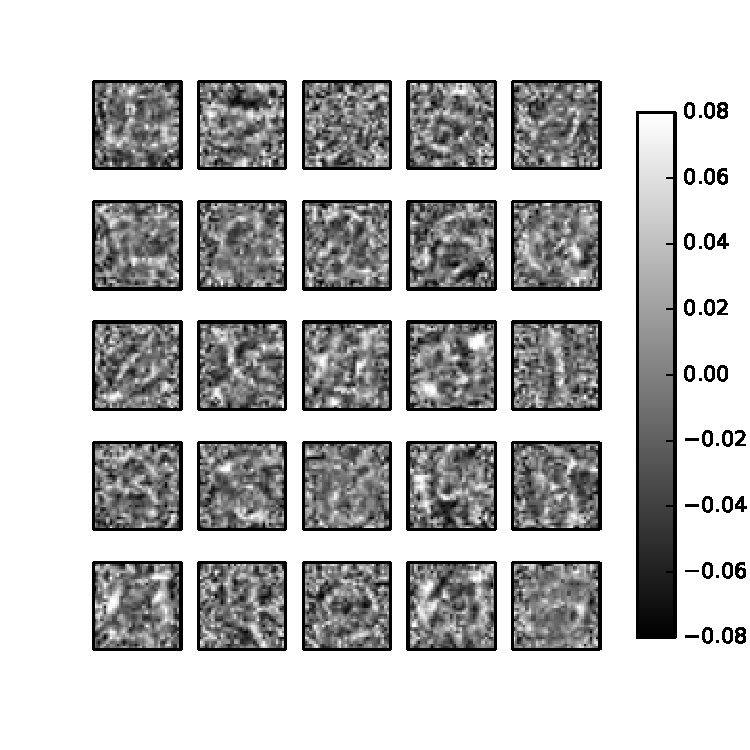
\includegraphics[width=0.5\textwidth]{weights_e0_60000}
	}
	\caption{Trained weights of MNIST training set.}
\end{figure}

\subsection{Reconstruction}
AE reconstructs visible units.
\begin{figure}
	\centering
	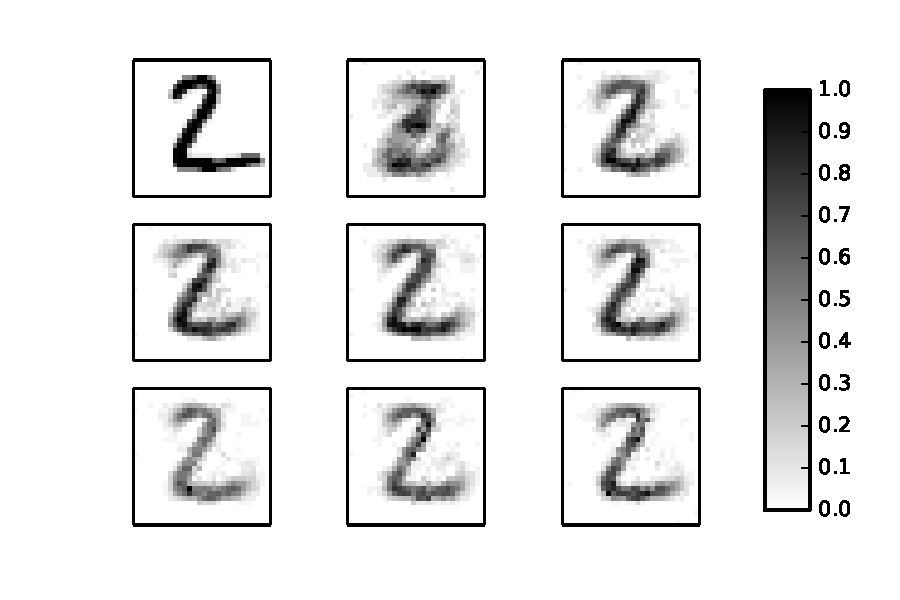
\includegraphics[width=0.5\textwidth]{recon_digit}
	\caption{Reconstructions of a testing digit `2' using trained weights during training.}
	\label{fig:recon}		
\end{figure}
\subsection{Classification Performance}
Compare CA of spiking AE with non-spiking continuous neurons. 
\begin{figure}
	\centering
	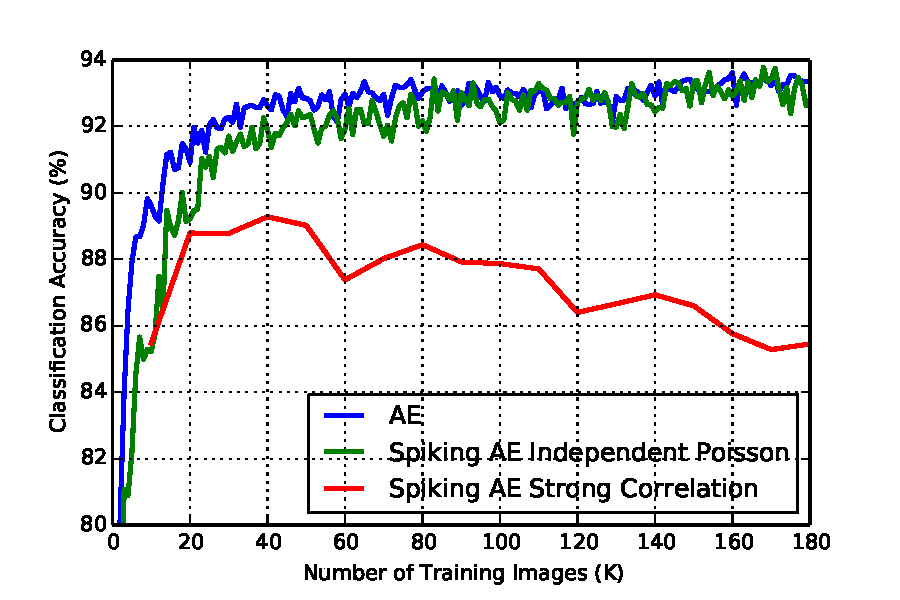
\includegraphics[width=0.5\textwidth]{recog_comp}
	\caption{Fast recognition with spiking neurons. Classification accuracy increases over presence period of an image.}
	\label{fig:recog_comp}		
\end{figure}

Fast classification.
\begin{figure}
	\centering
	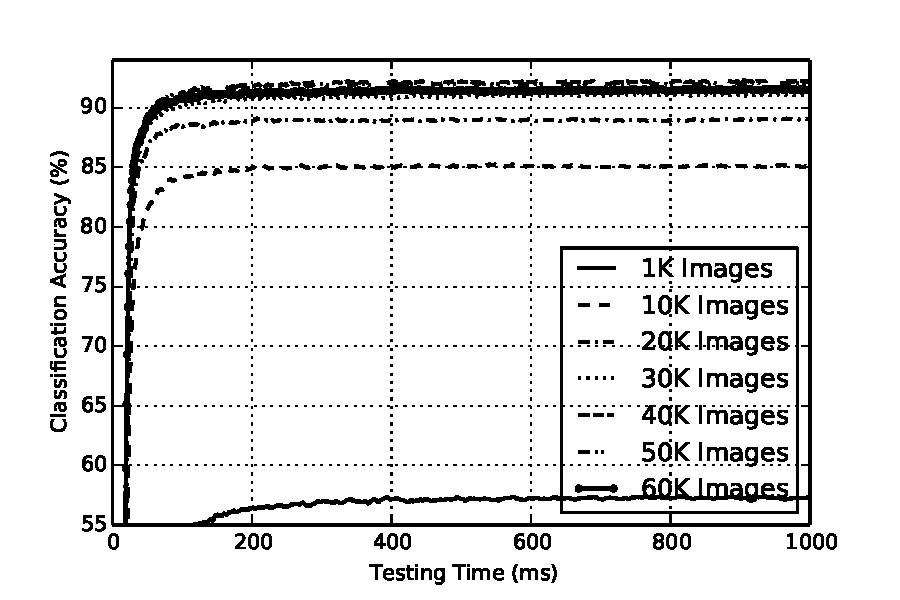
\includegraphics[width=0.5\textwidth]{recog_speed}
	\caption{Fast recognition with spiking neurons. Classification accuracy increases over presence period of an image.}
	\label{fig:recog_speed}		
\end{figure}


% An example of a floating figure using the graphicx package.
% Note that \label must occur AFTER (or within) \caption.
% For figures, \caption should occur after the \includegraphics.
% Note that IEEEtran v1.7 and later has special internal code that
% is designed to preserve the operation of \label within \caption
% even when the captionsoff option is in effect. However, because
% of issues like this, it may be the safest practice to put all your
% \label just after \caption rather than within \caption{}.
%
% Reminder: the "draftcls" or "draftclsnofoot", not "draft", class
% option should be used if it is desired that the figures are to be
% displayed while in draft mode.
%
%\begin{figure}[!t]
%\centering
%\includegraphics[width=2.5in]{myfigure}
% where an .eps filename suffix will be assumed under latex, 
% and a .pdf suffix will be assumed for pdflatex; or what has been declared
% via \DeclareGraphicsExtensions.
%\caption{Simulation results for the network.}
%\label{fig_sim}
%\end{figure}

% Note that the IEEE typically puts floats only at the top, even when this
% results in a large percentage of a column being occupied by floats.


% An example of a double column floating figure using two subfigures.
% (The subfig.sty package must be loaded for this to work.)
% The subfigure \label commands are set within each subfloat command,
% and the \label for the overall figure must come after \caption.
% \hfil is used as a separator to get equal spacing.
% Watch out that the combined width of all the subfigures on a 
% line do not exceed the text width or a line break will occur.
%
%\begin{figure*}[!t]
%\centering
%\subfloat[Case I]{\includegraphics[width=2.5in]{box}%
%\label{fig_first_case}}
%\hfil
%\subfloat[Case II]{\includegraphics[width=2.5in]{box}%
%\label{fig_second_case}}
%\caption{Simulation results for the network.}
%\label{fig_sim}
%\end{figure*}
%
% Note that often IEEE papers with subfigures do not employ subfigure
% captions (using the optional argument to \subfloat[]), but instead will
% reference/describe all of them (a), (b), etc., within the main caption.
% Be aware that for subfig.sty to generate the (a), (b), etc., subfigure
% labels, the optional argument to \subfloat must be present. If a
% subcaption is not desired, just leave its contents blank,
% e.g., \subfloat[].


% An example of a floating table. Note that, for IEEE style tables, the
% \caption command should come BEFORE the table and, given that table
% captions serve much like titles, are usually capitalized except for words
% such as a, an, and, as, at, but, by, for, in, nor, of, on, or, the, to
% and up, which are usually not capitalized unless they are the first or
% last word of the caption. Table text will default to \footnotesize as
% the IEEE normally uses this smaller font for tables.
% The \label must come after \caption as always.
%
%\begin{table}[!t]
%% increase table row spacing, adjust to taste
%\renewcommand{\arraystretch}{1.3}
% if using array.sty, it might be a good idea to tweak the value of
% \extrarowheight as needed to properly center the text within the cells
%\caption{An Example of a Table}
%\label{table_example}
%\centering
%% Some packages, such as MDW tools, offer better commands for making tables
%% than the plain LaTeX2e tabular which is used here.
%\begin{tabular}{|c||c|}
%\hline
%One & Two\\
%\hline
%Three & Four\\
%\hline
%\end{tabular}
%\end{table}


% Note that the IEEE does not put floats in the very first column
% - or typically anywhere on the first page for that matter. Also,
% in-text middle ("here") positioning is typically not used, but it
% is allowed and encouraged for Computer Society conferences (but
% not Computer Society journals). Most IEEE journals/conferences use
% top floats exclusively. 
% Note that, LaTeX2e, unlike IEEE journals/conferences, places
% footnotes above bottom floats. This can be corrected via the
% \fnbelowfloat command of the stfloats package.




\section{Conclusion}
The conclusion goes here.
Discussion about why divergence appear.



% conference papers do not normally have an appendix


% use section* for acknowledgment
\section*{Acknowledgment}
The research leading to these results has received funding from the European Research Council under the European Union's Seventh Framework Programme(FP/2007-2013) / ERC Grant Agreement n. 320689 and from the EU Flagship Human Brain Project (FP7-604102).





% trigger a \newpage just before the given reference
% number - used to balance the columns on the last page
% adjust value as needed - may need to be readjusted if
% the document is modified later
%\IEEEtriggeratref{8}
% The "triggered" command can be changed if desired:
%\IEEEtriggercmd{\enlargethispage{-5in}}

% references section

% can use a bibliography generated by BibTeX as a .bbl file
% BibTeX documentation can be easily obtained at:
% http://mirror.ctan.org/biblio/bibtex/contrib/doc/
% The IEEEtran BibTeX style support page is at:
% http://www.michaelshell.org/tex/ieeetran/bibtex/
%\bibliographystyle{IEEEtran}
% argument is your BibTeX string definitions and bibliography database(s)
%\bibliography{IEEEabrv,../bib/paper}
%
% <OR> manually copy in the resultant .bbl file
% set second argument of \begin to the number of references
% (used to reserve space for the reference number labels box)
%\begin{thebibliography}{1}
%
%\bibitem{IEEEhowto:kopka}
%H.~Kopka and P.~W. Daly, \emph{A Guide to \LaTeX}, 3rd~ed.\hskip 1em plus
%  0.5em minus 0.4em\relax Harlow, England: Addison-Wesley, 1999.
%
%\end{thebibliography}
\bibliography{ref}
\bibliographystyle{splncs03}


% that's all folks
\end{document}
